\documentclass[a4paper, 11pt, oneside]{report} 
\usepackage[utf8]{inputenc}
\usepackage[dutch]{babel}
\usepackage{amsmath}
\usepackage{amsfonts}
\usepackage{amssymb}
\usepackage{graphicx}
\usepackage{caption}
\usepackage[table,xcdraw]{xcolor}
\usepackage[toc,page]{appendix}
\usepackage{hyperref}
\usepackage{titlesec}
\usepackage{listings}
\usepackage{float}
\usepackage{tikz}
\usetikzlibrary{trees}
\usepackage{tikz-qtree}
\usepackage{graphicx}
\usepackage{fancyref}
\usepackage{wrapfig}
\usepackage{url}
\usepackage{pdflscape}
\usepackage{fancyvrb}
\usepackage{fancyhdr}
\graphicspath{ {Afbeeldingen/} }
\usepackage{subfig}
\usepackage{tabularx}
\usepackage{apacite}
\usepackage{longtable}
\usepackage{titlecaps}
%\usepackage[T1]{fontenc}
\usepackage{titlesec, blindtext, color}
\definecolor{gray75}{gray}{0.75}
\newcommand{\hsp}{\hspace{20pt}}
\usepackage{pdfpages}


\newcolumntype{L}[1]{>{\raggedright\arraybackslash}p{#1}}

\titleformat{\chapter}[hang]{\huge\bfseries}{\thechapter\hsp\textcolor{gray75}{|}\hsp}{0pt}{\Large\bfseries}

\def\figureautorefname{Figuur}
\def\sectionautorefname{Paragraaf}
\def\chapterautorefname{Hoofdstuk}
\def\tableautorefname{Tabel}
\DeclareRobustCommand{\VAN}[3]{#2} % set up for citation

%% Sets page size and margins 
\usepackage[a4paper,top=3cm,bottom=3cm,left=3cm,right=3cm,marginparwidth=1.75cm]{geometry}

\author{M.W.J. Berentsen}
\font\myfont=cmr12 at 40pt
\title{\myfont Drone meshnetwerk simulatie}
\usepackage{titling}

\newcommand{\subtitle}[8]{%
	\posttitle{%
		\par\end{center}
	\begin{center}\large#1\end{center}
	\vskip0.5em
	\begin{center}\large#2\end{center}
	\begin{center}\large#3\end{center}
	\begin{center}\large#4\end{center}
	\begin{center}\large#5\end{center}
	\begin{center}\large#6\end{center}
	\begin{center}\large#7\end{center}
	\begin{center}\large#8\end{center}
	\vskip0.5em}%
}

\subtitle{Software Design Document}{HAN Arnhem}{561399}{MWJ.Berentsen@student.han.nl}{Versie 1}{Alten Nederland B.V.}{Docent: J. Visch, MSc}{Assessor: ir. C.G.R. van Uffelen}

\setlength{\parindent}{0pt}
\setlength{\parskip}{5pt plus 2pt minus 1pt}



\hypersetup{colorlinks=true, urlcolor=red,citecolor=black,linkcolor=blue}  % Colours hyperlinks in blue, but this can be distracting if there are many links.
\setcounter{tocdepth}{2}



\begin{document}
\begin{figure}
	\begin{center}
\includegraphics[scale=0.1]{alten}\end{center}
\end{figure}
\maketitle

%\section*{Voorwoord}
%\addcontentsline{toc}{section}{\protect\numberline{}Voorwoord}
%\pagebreak

%Geschikt voor minimaal 50 nodes; Kan slecht of geen signaal nabootsen

\tableofcontents
\clearpage


%\clearpage

%\section*{Samenvatting}
%\addcontentsline{toc}{section}{\protect\numberline{}Samenvatting}
%\pagebreak


\chapter{Inleiding}
\label{inleiding}
Het volgende verslag betreft de Software Requirements Specification voor de afstudeerstage van Maurice Berentsen (hierna: student).
Dit document volgt het document: \textit{"Software Design Description Template"} \cite{template:sdd}

Het beschrijft TODO

\section{Overall Description}
\label{inleiding:omschrijving}
\section{Doel van dit document}
\label{inleiding:doel}
\section{Begrippenlijst}
\label{inleiding:begrippenlijst}

% Please add the following required packages to your document preamble:
% \usepackage[table,xcdraw]{xcolor}
% If you use beamer only pass "xcolor=table" option, i.e. \documentclass[xcolor=table]{beamer}
\begin{table}[H]
\centering

\label{begrippen}
\begin{tabular}{|l|l|}
\hline
\rowcolor[HTML]{C0C0C0}
Term        & Omschrijving                                                         \\ \hline
term        & Omschrijving                                                      	\\ \hline

\end{tabular}
\caption{Begrippenlijst}
\end{table}

\chapter{Architectural Overview}
\label{architectural}
\chapter{Detailed Design Description}
\label{DetailedDesign}
\section{Deployment Diagram}
\label{DetailedDesign:deployment}
\subsection{Design Decisions related to deployment}
\label{DetailedDesign:deployment:decisisions}
\section{Design Sub-Systeem Drone Simulatie}
\label{DetailedDesign:DroneSimumlatie}
\subsection{Design Class Diagram}
\label{DetailedDesign:DroneSimumlatie:class}
\begin{figure}[H]
	\begin{center}\includegraphics[width=\linewidth]{UML/out/DroneSimulation/class/DroneSimClass/DroneSimClass.png}\end{center}
	\caption{class diagram Drone Simulatie}
	\label{fig:class:dronesimulatie}
\end{figure}
\subsection{Sequence Diagrams}
\label{DetailedDesign:DroneSimumlatie:sequence}
\subsection{Activity and State Diagrams}
\label{DetailedDesign:DroneSimumlatie:Activity}
\subsection{Design decisions made for the sub-system}

\section{Design Sub-Systeem Meshnetwerk}
\label{DetailedDesign:MeshNetwerk}
\subsection{Design Class Diagram}
\label{DetailedDesign:MeshNetwerk:class}
\label{DetailedDesign:DroneSimumlatie:class}
\begin{figure}[H]
	\begin{center}\includegraphics[width=\linewidth]{UML/out/MeshNetwork/class/DroneSimClass/DroneSimClass.png}\end{center}
	\caption{class diagram Drone Simulatie}
	\label{fig:class:dronesimulatie}
\end{figure}
\subsection{Sequence Diagrams}
\label{DetailedDesign:MeshNetwerk:sequence}
\subsection{Activity and State Diagrams}
\label{DetailedDesign:MeshNetwerk:activity}
\subsection{Design decisions made for the sub-system}
\label{DetailedDesign:MeshNetwerk:decisions}

\section{Design Sub-System Wireless Simulatie}
\label{DetailedDesign:WirelessSimulatie}
\subsection{Design Class Diagram}
\label{DetailedDesign:WirelessSimulatie:class}
\subsection{Sequence Diagrams}
\label{DetailedDesign:WirelessSimulatie:sequence}
\subsection{Activity and State Diagrams}
\label{DetailedDesign:WirelessSimulatie:activity}
\subsection{Design decisions made for the sub-system}
\label{DetailedDesign:WirelessSimulatie:decisions}


\bibliographystyle{apacite}
\bibliography{bilbliography.bib}

\clearpage
\appendix
\chapter{Appendix 1}
\label{app:iteratieplan}





\end{document}